
\chapter{Getting started}
\label{txt:gettingstarted}

Once you have your Tellervo desktop application installed (see chapter \ref{txt:installation}) and you also have access to a Tellervo server (either via your lab network administrator or your own on as a Virtual Appliance) you are ready to start using Tellervo.  Below are some basic instructions for performing common tasks in Tellervo followed by a number of more in-depth chapters.

\section{Main window}

When you launch Tellervo in full mode and login you will be presented with the Tellervo main window (figure \ref{fig:mainwindow}).  The screen is split into two main areas.  On the left is a list of series that are currently loaded.  On the right are a series of tabs that display data and information about the currently selected series.  The tabs include:  

\begin{description}
\item[Data] -- This is the main tab for showing ring-width data for the currently selected series.  The tab is split into three: data tables contain the ring-width values; graph of the ring-widths; and a ring remarks panel where individual rings can be tagged with comments.
\item[Metadata] -- The metadata tab records all the associated information about the currently selected series following the Tree Ring Data Standard (TRiDaS).  Full details about metadata is given in chapter \ref{txt:metadata}.
\item[Components viewer] -- For series that are derived from other series e.g.\ indices, sums, chronologies etc, the components viewer displays all the series that are referenced by the currently selected series.
\item[Dependents viewer] -- Displays all other series that rely upon the currently selected series.  For instance if this series is used in one or more chronologies, then those chronologies will be displayed here.
\item[Map] -- Contains a 3D map viewer with the location of all the series currently loaded and that have location data recorded in their metadata.
\end{description}

\begin{figure}[hbtp]
  \centering
    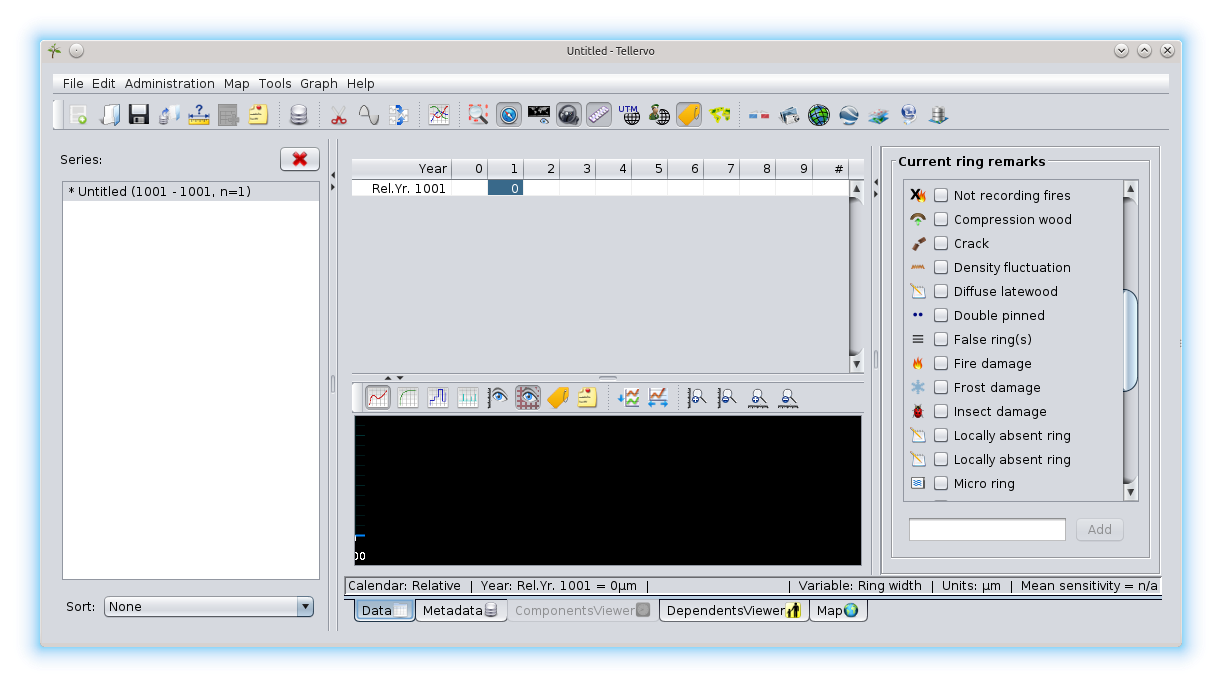
\includegraphics[width=\textwidth]{Images/mainwindow.png}
    \caption{The main window in Tellervo.  The screen is split into a two, with a list of open series in the workspace on the left, and a series of tabs on the right showing information about the currently selected series. The data tab is opened with a new series ready to receive measurements.}
    \label{fig:mainwindow}
\end{figure}


\section{Measuring a new sample}
\index{Sample!Measuring|(}
Once your measuring platform has been configured, measuring your first sample is simple.  To start a new measurement go to \menutwo{File}{New} or click the `new' icon on the toolbar. A dialog will appear where you can scan your sample's barcode, or press the button to enter metadata for your sample later. Barcodes minimize data entry errors and also speed up the process of measuring your samples. See section \ref{txt:barcodes} for more information. Once you have scanned your barcode or pressed the button, you will then be presented with an empty Tellervo metadata screen.

The next step is to fill out the metadata information. If you have used a barcode, nearly all of this metadata will be filled in for you, otherwise you will need to fill this out yourself. Details about metadata can be found in chapter \ref{txt:metadata}, page \pageref{txt:metadata}.  Once you have populated the metadata tab, you can then switch to the data tab.  


Before you begin measuring you need to tell Tellervo what sort of measurements you are making: whole ring widths; or early/latewood widths (the default is whole ring widths).  To specify early/latewood widths you need to go to \menuthree{Edit}{Measuring mode\ldots}{Early and latewood widths}.  If you use this menu after you have already measured some rings you will be warned that Tellervo will delete the data you have already collected.  Once in `early and latewood widths' measuring mode you will be able to choose which data is displayed in the table by clicking the variable box on the status line and choose between: Ring width; Earlywood width; Latewood width; Early/Latewood width.

To begin measuring your sample you can now go to \menutwo{Edit}{Start measuring}, press the start measuring button on the toolbar, or you can press F5. While measuring you should be provided with audible feedback for each ring measured with a more pronounced sound made every 10th ring. If there is a problem communicating with your measuring hardware, check your settings in the preferences dialog. If you still have problems contact the Tellervo developers by going to \menutwo{Help}{Report bug on last transaction}, making sure you include your email address and any further information.

If your sample is already dated and/or you already know how many rings your sample has, then you can initialise your data matrix using the button on the toolbar.  This gives you a dialog requesting date and ring number information which can be useful for those of you that use the skeleton plotting method prior to measuring.  

Note by default Tellervo labels rings as relative years beginning in 1001.  If your sample is dated, you should explicity tell Tellervo either using the initialise grid function prior to measuring, or by going to \menutwo{Tools}{Redate} once you've finished.

Depending on the measuring platform hardware you have, you will see some variation of the measuring panel in figure \ref{fig:measurepanel}. The left display holds the absolute position of the last ring boundary (for device that measure cumulatively), the middle display holds the last recorded measurement width and the right display holds the current position of the measuring plaform (for devices that report live measurements).  The right-hand display is useful for devices that don't have a physical display such as the Lintab. 

\begin{wrapfigure}{r}{0.5\textwidth}
  \begin{center}
    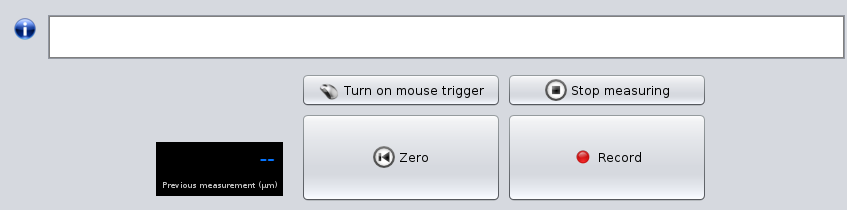
\includegraphics[width=70mm]{Images/measuringpanel.png}
  \end{center}
  \caption{Measuring control panel.  The number of digital displays will vary between 1 and 3 depending on what type of measuring platform hardware you have.}
  \label{fig:measurepanel}
\end{wrapfigure}


Tellervo supports the measuring of rings both individually and cumulatively.  We feel that it is easier and more accurate to measure rings individually, that is to say the device is reset to zero after each measurement.  If a device accepts requests to reset measurements (e.g.\ Quadra Chek boxes) or if it automatically resets itself to zero after recording a measurement (e.g.\ EVE IO) then this procedure is used by Tellervo.  In this case the user begins measuring by setting the display to zero, then turns the platform to the end of the ring, then either presses the `measure' button on the hardware device or the `record' button on the screen.

\tip{If your device does not have a physical `measure' button you don't need to click on the `record' button each time.  Instead click on the `turn on mouse trigger' button and then you can use your mouse's left button as a measure button regardless of where the mouse is on the screen. This means you don't need to lift your eyes from your microscope to ensure you are clicking the button correctly.  When you're finished measuring press escape to exit this mode.}

Certain devices (e.g.\ Boekler Microcode boxes) do not listen for requests to reset to zero.  In this case to measure each ring individually, you would need to manually reset the reading to zero following each measurement.  This would of course be extremely tedious.  In this situation Tellervo measures cumulatively from the beginning of the first ring and calculates the ring width based on the previous ring boundary position.  With this method you must be careful not to knock your sample, and you must also take special care when altering radii to navigate around problem structures.  If you do knock your sample, the best way to recover is to reset your platform to zero and press the measure button.  Next, press the `stop measuring button', manually fix the values in the data table, then begin measuring again from where you left off.


\begin{wrapfigure}{r}{0.45\textwidth}
  \begin{center}
    
\includegraphics[width=0.40\textwidth]{Images/ringremarks.png}
  \end{center}
  \caption{Right click context menu showing some of the options for adding remarks to rings.}
  \label{fig:ringremarks}
\end{wrapfigure}

If you are in `Early and latewood widths' measuring mode the measurements are made and sent to the data table in pairs.  The first measurement should be of the earlywood of the ring, and the next value the latewood measurement.  Whether you are currently measuring early or latewood is indicated as a message at the bottom of the measuring panel.

\index{Ring remarks}
While you measure your sample you can flag features in a ring by right clicking on any cell in the table and selecting one or more of the standard notes (see figure \ref{fig:ringremarks}).  

Tellervo supports all standard TRiDaS remarks including: fire damage; frost damage; crack; false ring(s); compression wood; tension wood; traumatic ducts; single pinned; double pinned; triple pinned and many others.  Rings that include remarks are indicated by the relevant icon in the data screen.  Depending on your method of work, this can be useful for keeping track of sample pin holes.  For instance, if a missing or false ring is discovered after a sample has been pinholed, the offset in pinholes can be easily seen without resurfacing the sample.  

In addition to the right click menu, you can also access ring remarks by opening the remarks panel using the button on the toolbar.  This panel gives the the ability to add free text remarks to individual rings.  One final method for adding remarks is specific to fire history researchers.  Standard FHX-style remarks can be added to rings by pressing the equivalent FHX character code key in the relevant ring cells.  For instance pressing a lower-case `a' in a cell will add the `fire injury in latewood' remark.   

The data screen also contains a status bar at the bottom. By clicking on the units section, you can switch between micron and 1/100th mm units. Tellervo understands the units being supplied by the measuring platform, therefore changes here are purely for display purposes only. If you have a platform that measures in microns, but prefer to see the values in 1/100th mm then you can use this feature.  There are also options on the status bar that enable you to choose one of a variety of summary statistics about your series.

Once you have finished measuring your sample, you should then go to \menutwo{File}{Save} to save your series to the database. 
\index{Sample!Measuring|)}


\section{Opening existing data}
\index{Sample!Opening}
If you have used traditional dendrochronology software, you are probably used to opening existing dendro data files from your computer.  Tellervo works in a different way.  All data accessed by Tellervo is stored within the central Tellervo database rather than in files.  The database provides many benefits over file based storage, most importantly it means there is a high degree of security and integrity in your data.\footnote{This doesn't mean you don't have to backup your data though!  Whoever is in charge of maintaining your Tellervo database should make sure regular backups are made--preferably offsite.}

To use data that you have stored in existing data files you must first \emph{import} your data into the Tellervo database.  This gives you the opportunity to clean-up your data!  For details of how to import your data see chapter \ref{txt:importExport}, page \pageref{txt:importExport}.

Once you have data in your database, either by importing existing data files or measuring new samples, you can access your data through the database browser.  This is accessed through the \menutwo{File}{Open} or \menutwo{File}{Open multiple} menus and an example of the dialog is shown in figure \ref{fig:dbbrowser}. The same database browser dialog is used in multiple places throughout Tellervo, e.g.\ when adding additional series to graphs and when choosing chronologies to crossdate against. 

\begin{figure}[hbtp]
  \centering
    
\includegraphics[width=0.9\textwidth]{Images/dbbrowser.png}
    \caption{Screenshot of the database browser dialog.}
    \label{fig:dbbrowser}
\end{figure}

The database browser is divided into two main parts.  On the left are the browse and search tabs, and on the right is the series table.  Selecting options in the browse or search tab populates the series table on the right with all the series that match the specified criteria.  

The browse tab shows a heirarchical tree view of the contents of your Tellervo database based upon the TRiDaS data model.  The panel will be pre-populated with all the objects in your database but it is possible to `drill-down' by right clicking on an object and choosing `Expand branch'.  Expanding an object for instance, will show all the elements associated with that object, and expanding an element will show all the samples associated with the specified element.  To better understand the TRiDaS terminology please read chapter \ref{txt:metadata}, page \pageref{txt:metadata}.

By double clicking (or right clicking and choosing `Search for associated series') on an item in the browse panel Tellervo will search the database for all series that are associated with the specified entity.  The results of the search will be shown in the series table on the right of the screen.  This table shows basic metadata about each search and is sortable by click on any of the column headers.  To open a series, simply select one of these series and click `OK'.  If the database browser is open in 'multiple series' mode, then you can use the arrow buttons to select multiple series to open in one go.

There is also a `Show options' button on the database browser dialog.  This adds additional advanced methods for filtering the series table to help you find the data you are interested in.

\index{Tags}
At the bottom of the list of objects in the browse tab are two categories of `tags': personal tags; and system tags.  The tagging concept in Tellervo is borrowed from the world of social media.  Just like you can tag a photo or blog post in social media tools with a tag, perhaps someone's name, a keyword, or location name, in Tellervo you can tag series.  For instance with tags like `needs checking', or `in progress'.  Any tags used will be displayed in the list and by double clicking on them, all series that have been tagged will be displayed.  Tags can be personal (only visible to you) or system tags.  The system tags are useful when you want to share tags with other users of your database.

\section{Reconciling data}
\index{Sample!Reconciling}
Tellervo has been developed not only for experience dendrochronologists, but as a tool for teaching students.  It therefore includes a comprehensive `reconciling' tool for supervisors to check the quality of measurements made by students.  The reconcile dialog does a comparison of a measurement series made by a student with a references series of the same radius measured by the supervisor.  The same dialog can also prove useful for comparing measurements from two experienced dendrochronologists when handling particularly difficult samples.

Open the series you would like to check as normal.  Next go to \menutwo{Tools}{Reconcile}.  This will open a database browser window where you should then locate the reference series you'd like to compare against.  The two series will then be opened in a reconcile window such as the one shown in figure \ref{fig:reconcile}.

\begin{figure}[hbtp]
  \centering
    
\includegraphics[width=\textwidth]{Images/reconcile.png}
    \caption{Example of the reconcile window showing the differences between two dummy datasets.  The green cells show where the series are in agreement, and the red cells and cell-pairs with red borders are where there are conflicts.}
    \label{fig:reconcile}
\end{figure}

The reconcile window contains: a data table for each of the series; a graph of the two series; and an information panel describing inconsistencies.  The reconcile tool runs a number of tests:

\begin{description}

\item[Series length] -- this simply test checks that the two series are the same length
\item[Trend agreement]  -- this checks that the trend from year $n$ to $n+1$ is in agreement between the two series.  For example if the ring-widths increase from 1950 to 1951 in the reference series then they should also increase in the test series.  Where trends are different the pair of years are marked with a red border.
\item[Error margin] -- this checks that the ring-width values in the reference and test series are within a 3\% error margin.  Where the ring-widths are outside this error margin, then cells are coloured red.
\end{description}

In circumstances where the test series includes an extra, or is missing a ring then typically there will be a large amount of `red' in the tables begin at the point of the error.  Such errors are typically easiest seen in the graph.  

Errors in the measurements can be fixed from within the reconciliation screen by directly editing the data tables.  Right click popup menus can be used to insert or delete rings where necessary.  There is also the option of remeasuring the current ring.  The remeasuring tool allows you to remeasure the same ring multiple times to triple check you end up with an accurate measurement.

Once you have fixed all the errors you can then click the `finish' button to commit the changes to the test series.

